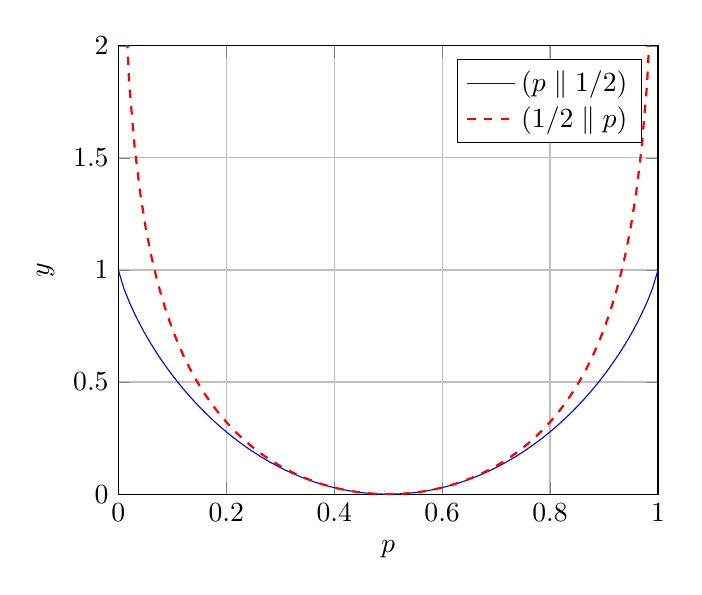
\begin{tikzpicture}
  \begin{axis}[
    xlabel=$p$,
    ylabel=$y$,
    xmin=0, xmax=1,
    ymin=0, ymax=2,
    legend pos=north east,
    grid=both,
    ]
    
    % Function  p * log2(2 * p) + (1 - p) * log2(2 * (1 - p))
    \addplot[blue, domain=0:1, samples=100] {x * log2(2 * x) + (1 - x) * log2(2 * (1 - x))};
    \addlegendentry{$\dkl(p \parallel 1/2)$}
    
    % Function 0.5 * (log2(1 / (2 * p)) + log2(1 / (2 * (1 - p))))
    \addplot[red, domain=0:1, samples=100, dashed, thick] {0.5 * (log2(1 / (2 * x)) + log2(1 / (2 * (1 - x))))};
    \addlegendentry{$\dkl(1/2 \parallel p)$}
    
  \end{axis}
\end{tikzpicture}